\documentclass[a4paper,12pt]{article}

\usepackage{amsmath,amsthm,ae,aecompl,sgame,natbib,sgamevar}
\usepackage[margin=2.5cm]{geometry}
\usepackage{tikz}
\usetikzlibrary{trees}

\title{Exercises Adv. Micro II}
\author{Christoph Schottm\"uller}

\begin{document}

\maketitle

\section{Rationalizability}
\begin{enumerate}
\item %Come up with a three player game in which each player has two actions and the actions surviving iterative elimination of strictly dominated strategies is not the same as the set of rationalizable actions.
  Show that in the following three player game (only payoffs of player 1 are given), $M$ is a never best response although $M$ is not strictly dominated.
\begin{table}[h]
    \centering
    \begin{tabular}{l|c|c}
      & L &R\\ \hline
      U& 10,  &10, \\
      M&6,  &0, \\
      D& 0, & 10,
    \end{tabular}
    $\qquad$
    \begin{tabular}{l|c|c}
      & L &R\\ \hline
      U& 10,  &0,  \\
      M&0,&6, \\
      D& 10, & 10,
    \end{tabular}
    \caption{P1 chooses row, P2 column, P3 table}
    \label{tab:domVsRatio}
  \end{table}
  
\item Show that the order of elimination does not matter for the outcome of iterative elimination of strictly dominated strategies. \\(Hint: Consider two orders, say A and B, and suppose they lead to different outcomes. Consider then the first action to be deleted in one procedure, say A, while surviving the other, i.e. B. Show that this action is strictly dominated at the end of procedure B which yields the desired contradiction.)
\item (Numerical) Consider two players participating in a lab experiment. The monetary payoffs the two players get from the experimenter when choosing their strategies are given in table \ref{tab:monRatio}. (note: this time the numbers in the table are not utilities but amounts of money!) Assume that players are only interested in their own monetary payoffs and not in the monetary payoffs for the other players.
  \begin{table}[h]
    \centering
    \begin{tabular}{l|c|c}
      & L &R\\ \hline
      U& 3,1  &0,0  \\
      M1&1,0&1,1 \\
      M&2.6,0  &0.5,0 \\
      D& 0,1 & 3,0
    \end{tabular}
    \caption{Monetary payoff}
    \label{tab:monRatio}
  \end{table}
  \begin{enumerate}
  \item Suppose players value money linearly $u_i(x)=x$ for any monetary amount $x$. Which actions are rationalizable?
  \item Suppose players value money  $u_i(x)=-e^{-r x}$ for any monetary amount $x$. Which actions are rationalizable if the parameter $r$ is very high? (you can choose a high number like $3$ and check)
     \item Suppose players value money $u_i(x)=e^{r x}$ for any monetary amount $x$. Which actions are rationalizable if the parameter $r$ is very high?
     \end{enumerate}
     What is the interpretation in terms of risk preferences? (see \cite{weinstein2016effect} for more on this topic)
\end{enumerate}


\section{Existence of Nash equilibrium}
\label{sec:nash-theorem-fixed}

\begin{enumerate}
\item Show that a pure strategy Nash equilibrium exists in the following two player game: $I=\{P1,P2\}$, $S_1=S_2=[0,1]$, $u_i(s_i,s_{-i})$ is differentiable and strictly (quasi-)concave in $s_i$ and $\partial u_i/\partial s_i$ is continuous in both variables.\\
  (Hint: Show that the first order condition leads to a continuous best response function. Then, verify that the two best response functions must intersect.)
\end{enumerate}

\section{Correlated equilibrium}
\label{sec:corr-equil}
\begin{enumerate}
\item Find a correlated equilibrium that yields a higher payoff to every player than the unique Nash equilibrium (game in table \ref{tab:corEq}).
   \begin{table}[h]
\centering
 \begin{game}{3}{3}
       \> L \> C \>R\\ %\hline
U   \>1,1   \> 2,4 \> 4,2   \\
M   \>4,2   \> 1,1 \> 2,4 \\
D  \> 2,4    \>4,2  \>1,1
\end{game}  
\caption{correlated equilibrium}
\label{tab:corEq}
\end{table}
\item In the example from the lecture (using in particular the inequalities on slide 9), show that the set of correlated equilibria is the set of all probability distributions $(p_{UL},p_{UR},p_{DL},p_{DR})$ for which the the probability on each pure Nash equilibrium is at least as high as the probability on any other strategy profile. (Note: This is \emph{not} a general result!) Given this, derive the correlated equilibrium with the lowest and the highest sum of payoffs. 
\end{enumerate}

\section{Bayesian Nash equilibrium}
\label{sec:Bayes-nash-eq}
\begin{enumerate}
\item Two player Cournot with uncertain costs: Payoffs of player $i$ are $(\theta _i-q_1-q_2)q_i$ where $\theta _i$ is the difference between the intercept of a linear demand function and costs. It is commonly known that $\theta _1=1$. However, $\theta _2$ is private information of firm 2. Firm 1's (commonly known) belief is that $\theta _2$ is $3/4$ with probability $1/2$ and $5/4$ with probability $1/2$.
  \begin{enumerate}
  \item If firm 1's equilibrium quantity is $q_1^*$, what is firm 2's best response?
  \item If type $j\in\{l,h\}$ of firm 2 produces quantity $q_2^j$, what is firm 1's best response quantity? (i.e. maximizing expected payoff)
    \item What is the BNE of this game?
  \end{enumerate}
\item Purification: Consider the game in table \ref{tab:purify}. Let $\theta _i$ be private information and be distributed uniformly on $[0 ,\varepsilon ]$. Assuming $\varepsilon >0$ sufficiently small, derive a BNE in cutoff strategies; i.e. P1 (P2) plays U (L) if $\theta _1>\bar{\theta }_1$ ($\theta _2>\bar{\theta }_2$) and D (R) otherwise for some $\bar \theta_i\in(0,\bar{\varepsilon })$. Compare the equilibrium in the limit as $\varepsilon \rightarrow 0$ to the mixed strategy equilibrium in the game without private information (i.e. the game where $\theta _i=0$ is commonly known). 
     \begin{table}[h]
\centering
 \begin{game}{2}{2}
       \> L  \>R\\ %\hline
U   \>5$+\theta_1$,1$+\theta _2$    \> $\theta_1$,0   \\
D  \> 4,4$+\theta _2$    \>1,5
\end{game}  
\caption{purification}
\label{tab:purify}
\end{table}
\end{enumerate}

\section{Auctions}
\label{sec:auctions}

\begin{enumerate}

\item Take the first price sealed bid auction in the independnet private value framework. The purpose of this exercise is to show that in every BNE, the bidding strategy of an arbitrary bidder $i$ is weakly increasing in his valuation. Take two values $v_i^h$ and $v_i^l$ with $v_i^h>v_i^l$ and let $s_i()$ be an equilbrium strategy of player $i$.
  \begin{enumerate}
  \item In equilibrium type $v_i^l$ must prefer bidding $s_i(v_i^l)$ to bidding $s_i(v_i^h)$. Write down the corresponding inequality.
    % (v_i^l-s_i(v_i^l))*prob(win,s_i(v_i^l))\geq (v_i^l-s_i(v_i^h))*prob(win,s_i(v_i^h))
  \item In equilibrium type $v_i^h$ must prefer bidding $s_i(v_i^h)$ to bidding $s_i(v_i^l)$. Write down the corresponding inequality.
    % (v_i^h-s_i(v_i^h))*prob(win,s_i(v_i^h))\geq (v_i^h-s_i(v_i^l))*prob(win,s_i(v_i^l))
  \item Use the two inequality to show that $s_i(v_i^h)\geq s_i(v_i^l)$. (Hint: Note that bidding higher increases the probability of getting the object in a first price auction!)
    % adding inequalities gives: $(v_i^h-v_i^l) (prob(win,s_i(v_i^h))-prob(win,s_i(v_i^l))\geq 0$ which is only true if $s_i(v_i^h)\geq s_i(v_i^l)$
  \end{enumerate}
  
% \item Two people have to decide who gets an indivisible item. Their valuations of the item are private information and we regard the two $v_i$ as drawn independently from a uniform distribution on $[0,1]$. The two people have come up with the following auction mechanism: They simultaneously state a bid $b_i$ and the one stating the higher bid gets the item but has to pay half of his bid to the other player.
%   \\
%   Assume that there is a symmetric equilibrium of this game in which players bid according to a strictly increasing strategy $s(v)$. (If you find this hard, assume that $s(v)=\alpha v$ for some $\alpha>0$ and determine below the $\alpha$ for which this is an equilibrium.)
%   \begin{enumerate}
%   \item Write down the expected payoff of a player bidding $b$ (given that the other player bids according to $s$). (Hint: Do not forget that he might receive a payment from the other player!)
%     % $\int_0^{t(b)}v_i-b/2 \,dv_j+\int_{t(b)}^1 s(v_j)/2\,dv_j$
%   \item Derive the first order condition of an optimal bid.
%     % $t'(b)(v_i-b/2)-t(b)/2-t'(b) b/2=0$
%   \item What is the equilibrium bidding strategy? Why is it not optimal to bid your true valuation?
%     % use $t(b)=v_i$, $b=s(v_i)$ and $t'(b)=1/s'(v_i)$ in foc to get $(v_i-s(v_i))/(s'(v_i))-v/2=0$ which is solved by $s(v_i)=v_i*2/3$
%   \end{enumerate}
\item A buyer's valuation is uniformly distributed on $[0,1]$ and the buyer's private information. A seller's cost is also uniformly distributed on $[0,1]$ and the seller's private information. The buyer states an ask price $b_b$ and the seller simultaneously states an offer price $b_s$. If $b_s<b_b$, trade takes place at price $(b_s+b_b)/2$ while otherwise trade does not take place.
  \begin{enumerate}
  \item Explain/show why $b_s(c)=c$ and $b_b(v)=v$ is not an equilibrium although it would maximize welfare. 
  \item Show that the following is an equilibrium for any given $p\in[0,1]$:
    \begin{equation*}
      b_b(v)=
      \begin{cases}
        p & \text{ if }v\geq p\\
        0 & \text{ else }
      \end{cases}
    \qquad
      b_s(c)=
      \begin{cases}
        p & \text{ if }c\leq p\\
        1 & \text{ else }.
      \end{cases}
    \end{equation*}
    \item Suppose that players use linear strategies $b_b(v)=\alpha+\beta v$ and $b_s(c)=\gamma+\delta c$. Taking the strategy of the other player derive the best response of a seller/buyer with valuation $v$ / cost $c$. For which values of $\alpha,\beta,\gamma,\delta$ form the linear strategies an equilibrium?
    \end{enumerate}
  \item Two players participate in a contest: Each player chooses an effort level $e_i$. Effort is costly and reduces player $i$'s payoff by  $\theta _ie_i$. The player who choose the highest effort wins a prize of value 1. That is, the winner has payoff $1-\theta _i e_i$ while the loser has payoff $-\theta _i e_i$. The $\theta _i$ are private information and each player views the other player's type as being uniformly distributed on $[0.1,1.1]$. \\
    Write player $i$'s maximization problem given that the other player uses a strictly decreasing strategy $s$ (with inverse $t$). Derive the first order condition for optimal effort choice. Solve for a symmetric equilibrium in strictly decreasing strategies.
    % $\max_{e}(1.1-t(e))-\theta _i e$ where $t$ is the inverse of the other player's strategy $s$. Foc: $-t'(e)-\theta _i=0$, in equilibrium $t'(e(\theta _i))=1/s'(\theta _i)$ and we get $s'(\theta _i)=-1/\theta _i$. Using $s(1.1)=0$, we get $s(\theta _i)=\int_{\theta _i}^{1.1}1/x \,dx=log(1.1)-log(\theta _i)$
    (More on such contests can be found in \cite{moldovanu2001optimal}.)
\end{enumerate}

\section{Subgame perfect Nash equilibrium}
\label{sec:subgame-perfect-nash}

\begin{enumerate}
\item $I$ Players play the same strategic form game $\Gamma=[I,\{S_i\},\{u_i\}]$ $T$ times. Players observe immediately after each round $t=1,\dots, T$ which actions were chosen by the other players. Assume that $\Gamma$ has a unique Nash equilibrium $\sigma$. Show that the extensive form game $\Gamma_E$ formed by the $T$ time repetition of $\Gamma$ has a unique subgame perfect Nash equilibrium. (extra exercise: find an example $\Gamma$ with a unique NE in which $\Gamma_E$ has several NE that are not subgame perfect.)
  % add a "total destruction" action yielding for both players -1000 to a normal prisoner's dilemma and let $T=2$; the strategy cooperate in 1; defect in 2 if cooperation in 1 and total destruction otherwise is a NE but not subgame perfect
\end{enumerate}

\section{Weak PBE and sequential equilibrium}
\label{sec:weak-pbe-sequential}

\begin{enumerate}
\item Find a pure strategy NE in the game of figure \ref{fig:selten_ex}. Show that this NE is subgame perfect but not sequentially rational. Find a weak PBE. (Hint: use mixed strategies)
   \begin{figure}[h]
\centering
% First, set the overall layout of the tree
% You might need to play with these sizes to ensure nothing overlaps.
\tikzstyle{level 1}=[level distance=1.5cm, sibling distance=6cm]
\tikzstyle{level 2}=[level distance=1.5cm, sibling distance=2.5cm]
\tikzstyle{level 3}=[level distance=1.5cm, sibling distance=2cm]
\tikzstyle{level 4}=[level distance=1.5cm, sibling distance=1.5cm]
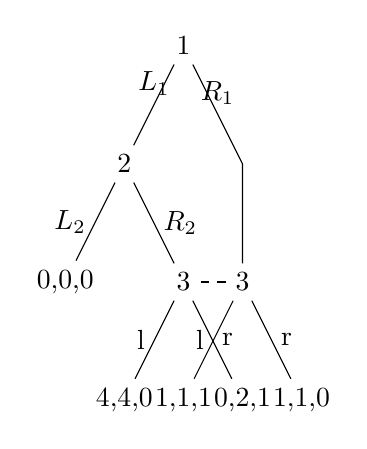
\begin{tikzpicture}
%Start with the parent node, and slowly build out the tree
% with each "child" representing a new level of the diagram
% each "node" represents a labelled (or unlabeled if you 
% want) node in the diagram.
\node{1}
    child{
             node{2}
             child{
               node{0,0,0}
             edge from parent
             node[left]{$L_2$}}
             child{
               node(b){3}
                  child{
               node{4,4,0}
               edge from parent
               node[left]{l}
               }
             child{
               node{0,2,1}
               edge from parent
               node[right]{r}
               }
                edge from parent
                node[right]{$R_2$}
               }
           edge from parent
           node[left,above]{$L_1$}
           }
    child{
           child{
               node(c){3}
                  child{
               node{1,1,1}
               edge from parent
               node[left]{l}
               }
             child{
               node{1,1,0}
               edge from parent
               node[right]{r}
               }
               }
         edge from parent
         node[right,above]{$R_1$}
         };
\draw [dashed](c)--(b);
\end{tikzpicture}
\caption{Selten's horse}
\label{fig:selten_ex}
\end{figure}

\item Consider the two games in figures \ref{fig:seq_eq_coalescing} and \ref{fig:seq_eq_coalescing2}. To what extent are these games different or the same? Show that there is a pure strategy sequential equilibria in figure \ref{fig:seq_eq_coalescing} that does not exist in \ref{fig:seq_eq_coalescing2}. Would this also be true for  weak PBE instead of sequential equilibrium?
% (R,r) supported by belief (0,1) is seq eq in first game but there is no equivalent in the second as A strictly dominates B and therefore seq rationality requires P1 to play A instead of B in the subgame. For any completely mixed strat converging to ?A P2's belief must be (1,0) and therefore his action in seq eq is l which means (LA,l) is unique seq eq in second game. Note that (RA,r) with belief (0,1) is still a weak PBE as P2's info set in never reached.
  
   \begin{figure}[h]
\centering
% First, set the overall layout of the tree
% You might need to play with these sizes to ensure nothing overlaps.
\tikzstyle{level 1}=[level distance=1.5cm, sibling distance=3.5cm]
\tikzstyle{level 2}=[level distance=1.5cm, sibling distance=1.5cm]
\tikzstyle{level 3}=[level distance=1.5cm, sibling distance=2cm]
\tikzstyle{level 4}=[level distance=1.5cm, sibling distance=1.5cm]
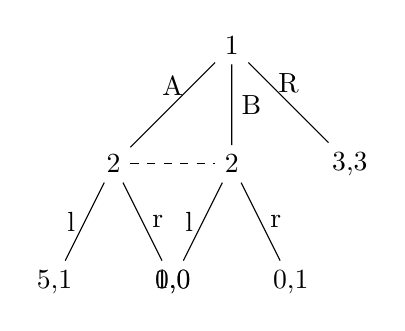
\begin{tikzpicture}
%Start with the parent node, and slowly build out the tree
% with each "child" representing a new level of the diagram
% each "node" represents a labelled (or unlabeled if you 
% want) node in the diagram.
\node{1}
             child{
               node(a){2}
                  child{
               node{5,1}
               edge from parent
               node[left]{l}
               }
             child{
               node{1,0}
               edge from parent
               node[right]{r}
               }
               edge from parent
               node[left,above]{A}
               }
             child{
               node(b){2}
                  child{
               node{0,0}
               edge from parent
               node[left]{l}
               }
             child{
               node{0,1}
               edge from parent
               node[right]{r}
               }
               edge from parent
               node[right]{B}
               }
    child{
         node{3,3}
         edge from parent
         node[right, above]{R}
         };
\draw [dashed](a)--(b);
\end{tikzpicture}
\caption{sequential equilibrium and coalescing moves}
\label{fig:seq_eq_coalescing}
\end{figure}

 \begin{figure}[h]
\centering
% First, set the overall layout of the tree
% You might need to play with these sizes to ensure nothing overlaps.
\tikzstyle{level 1}=[level distance=1.5cm, sibling distance=3.5cm]
\tikzstyle{level 2}=[level distance=1.5cm, sibling distance=3.5cm]
\tikzstyle{level 3}=[level distance=1.5cm, sibling distance=2cm]
\tikzstyle{level 4}=[level distance=1.5cm, sibling distance=1.5cm]
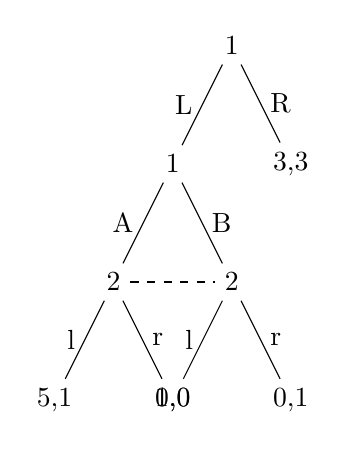
\begin{tikzpicture}
%Start with the parent node, and slowly build out the tree
% with each "child" representing a new level of the diagram
% each "node" represents a labelled (or unlabeled if you 
% want) node in the diagram.
\node{1}
    child{
             node{1}
             child{
               node(a){2}
                  child{
               node{5,1}
               edge from parent
               node[left]{l}
               }
             child{
               node{1,0}
               edge from parent
               node[right]{r}
               }
               edge from parent
               node[left]{A}
               }
             child{
               node(b){2}
                  child{
               node{0,0}
               edge from parent
               node[left]{l}
               }
             child{
               node{0,1}
               edge from parent
               node[right]{r}
               }
               edge from parent
               node[right]{B}
               }
           edge from parent
           node[left]{L}
           }
    child{
         node{3,3}
         edge from parent
         node[right]{R}
         };
\draw [dashed](a)--(b);
\end{tikzpicture}
\caption{game above with additional move}
\label{fig:seq_eq_coalescing2}
\end{figure}

\end{enumerate}

\bibliographystyle{chicago}
\bibliography{/home/christoph/stuff/bibliography/references.bib}

\end{document}
